\documentclass[smaller]{beamer}
\usepackage[utf8]{inputenc}
\usepackage{polski}
% \usepackage{color}
\usepackage{transparent}
\usepackage{amsrefs}
\usepackage{amsfonts}
\usepackage{listings}
\usepackage{syntax}
\usepackage{wrapfig}
\usepackage{graphicx}
\usepackage{caption}
\usepackage{subcaption}

\graphicspath{{includes/}}

\definecolor{javared}{rgb}{0.6,0,0} % for strings
\definecolor{javagreen}{rgb}{0.25,0.5,0.35} % comments
\definecolor{javapurple}{rgb}{0.5,0,0.35} % keywords
\definecolor{javadocblue}{rgb}{0.25,0.35,0.75} % javadoc

 \lstloadlanguages{
         Java
 }
 \lstset{language=Java,
%          basicstyle=\footnotesize\ttfamily, % Standardschrift
         basicstyle=\footnotesize\ttfamily, % Standardschrift
         %numbers=left,               % Ort der Zeilennummern
         numberstyle=\tiny\color{black},          % Stil der Zeilennummern
         stepnumber=1,               % Abstand zwischen den Zeilennummern
         numbersep=5pt,              % Abstand der Nummern zum Text
         tabsize=3,                  % Groesse von Tabs
% 	inputencoding=utf8, extendchars=\true
         extendedchars=true,         %
         breaklines=true,            % Zeilen werden Umgebrochen
keywordstyle=\color{javapurple}\bfseries,
stringstyle=\color{javared},
commentstyle=\color{javagreen},
morecomment=[s][\color{javadocblue}]{/**}{*/},
    		frame=b,         
 %        keywordstyle=[1]\textbf,    % Stil der Keywords
 %        keywordstyle=[2]\textbf,    %
 %        keywordstyle=[3]\textbf,    %
 %        keywordstyle=[4]\textbf,   \sqrt{\sqrt{}} %
         stringstyle=\color{blue}\ttfamily, % Farbe der String
         showspaces=false,           % Leerzeichen anzeigen ?
         showtabs=false,             % Tabs anzeigen ?
         xleftmargin=10pt,
         framexleftmargin=10pt,
         framexrightmargin=5pt,
         framexbottommargin=4pt,
         %backgroundcolor=\color{lightgray},
         showstringspaces=false      % Leerzeichen in Strings anzeigen ?        
 }
    %\DeclareCaptionFont{blue}{\color{blue}} 

  %\captionsetup[lstlisting]{singlelinecheck=false, labelfont={blue}, textfont={blue}}
  \usepackage{caption}
\DeclareCaptionFont{white}{\color{white}}
\DeclareCaptionFormat{listing}{\colorbox[cmyk]{0.43, 0.35, 0.35,0.01}{\parbox{\textwidth}{\hspace{15pt}#1#2#3}}}
\captionsetup[lstlisting]{format=listing,labelfont=white,textfont=white, singlelinecheck=false, margin=0pt, font={bf,footnotesize}}


\usetheme{Warsaw}
\title[Implementacja architektury usługowej]{Implementacja architektury usługowej - od specifikacji do kodu}
\author{Paweł Cesar Sanjuan Szklarz}
\institute{Warszawa Java User Group}
\date{5 czerwca 2012}
\begin{document}

\begin{frame}
\titlepage
\end{frame}


\begin{frame}
 \tableofcontents
\end{frame}

\section{Dependency Injection}
\subsection{Zasada działania}

\begin{frame}{\lstinline|DepencencyInjection implements InverseOfControl<new>|}
(IoC) Odwrócenie sterowania dla \lstinline|new|:
\begin{description}
 \item[odbieramy sterowanie] \hfill \\
 W kodzie nie występuje słowo kluczowe \lstinline|new|
 \item[przejmujemy sterowanie] \hfill \\
 Tworzenie instancji zgodnie z wydzieloną konfiguracją 
\end{description}
\end{frame}

\begin{frame}[fragile]{Injection points}
\begin{lstlisting}
public class DependencyInjectionPoints implements FeatureSpecification {
	@Inject
	private InjectionPointField field;
	@Inject
	@Named("custom key")
	private InjectionPointField fieldWithAnnotatedKey;
	private final InjectionPointConstructor fromConstructor;

	@Inject
	public DependencyInjectionPoints(InjectionPointConstructor constArgument) {
		super();
		this.fromConstructor = constArgument;
	}
}

\end{lstlisting}
% \lstinputlisting[label=UserServiceSimple,caption=Injection Points]{../../srcAPI/doc/wjug/DependencyInjectionPoints.java}
\end{frame}

\subsection{Słownik}
\begin{frame}[fragile]{Model ``explicit'' dla Injektowania zależności}

\begin{description}
 \item[Klucz] \hfill \\ 
 \lstinline|Key<T>|  =  \lstinline|Type<T>| $\times$ \lstinline|Annotation|
 \item[Injection Point] \hfill \\
 Położenie o kodzie $\rightarrow$\lstinline|Key<T>|
 \item[Dostawca]  \hfill \\
 \lstinline|public interface Provider<T> { T get(); }|
 \item[BindingProvider] (\lstinline|Injector|) \hfill \\
\begin{lstlisting}
public interface BindingProvider {
  <T> Provider<T> getProvider(Key<T> key);
}
\end{lstlisting}
\end{description}
\end{frame}

\begin{frame}{Algorithm tworzenia instancji}
 \begin{enumerate}
  \item<1-> \lstinline|Injector.createInstance(Key<T>)|
  \item<2-> \lstinline|Key<T>| $\rightarrow$ \lstinline|Provider<T>|
  \item<3-> \lstinline|Provider<T>| $\rightarrow$ Injection Point
  \item<4->  Injection Point $\rightarrow$ \lstinline|Key<T>|
  \item<5->  Powtarzamy ....
  \item<6->  Powstaje graf zależności przy tworzeniu instancji danego \lstinline|Key<T>|: \\
\lstinline|Key<T>| $\rightarrow$ \lstinline|Set<Provider<T>>|

 \end{enumerate}
\end{frame}

\subsection{Moduły Guice}
\begin{frame}{Uporządkowanie konfiguracji w modułach}
Moduł Guice to konfiguracja kilku kluczy w jednej klasie
\lstinputlisting[caption=Module]{../../srcAPI/doc/wjug/ModuleExample.java}
\end{frame}

\begin{frame}[fragile]{Zakres modułu}
Jeden moduł określa ``bindowanie'' dla zestawu kluczy:
\begin{lstlisting}[mathescape]
Modul = { Key<T> $\rightarrow$ Provider<T> }
\end{lstlisting}


Do tworzenia ``Injector'' potrzebujemy zestaw modułów tak, aby graf zależności był dobrze zdefiniowany:
\begin{lstlisting}
 Injector injector = Guice.createInjector(Module... modules);
\end{lstlisting}

% \lstinline|Injector injector = Guice.createInjector(Module... modules);|

\end{frame}

\section{Definicja architektury}
\subsection{Specifikacja usługi - Kategorie - Architektura}
\begin{frame}{Budowanie definicji architektury}

Usługa to kontrakt zdefiniowany przez zbiór interfejsów.

\pause

Architektura jest to struktura uporządkowująca zbiór usług.

\begin{description}
 \item[Specykacja usługi] Zbiór intejfejsów
 \item[Kategoria] Rozłączne zbiory usług 
 \item[Architektura] Zbiór wszystkich kategorii.
\end{description}

\pause
Definiujemy ograniczenia dla implementacji usług

\begin{description}
 \item[Implementacja] Bindowanie interfejsów usługi  (moduł Guice)
 \item[Relacja dostępności kategorii] Odpowiada na pytanie: \hfill \\
 Jakie \lstinline|Key<T>| mogę injektować w implementacji usługi?
\end{description}
\end{frame}

\subsection{Implementacje usług}
\begin{frame}{Specyfikacja-Kontrakt}
\begin{figure}
 \centering
 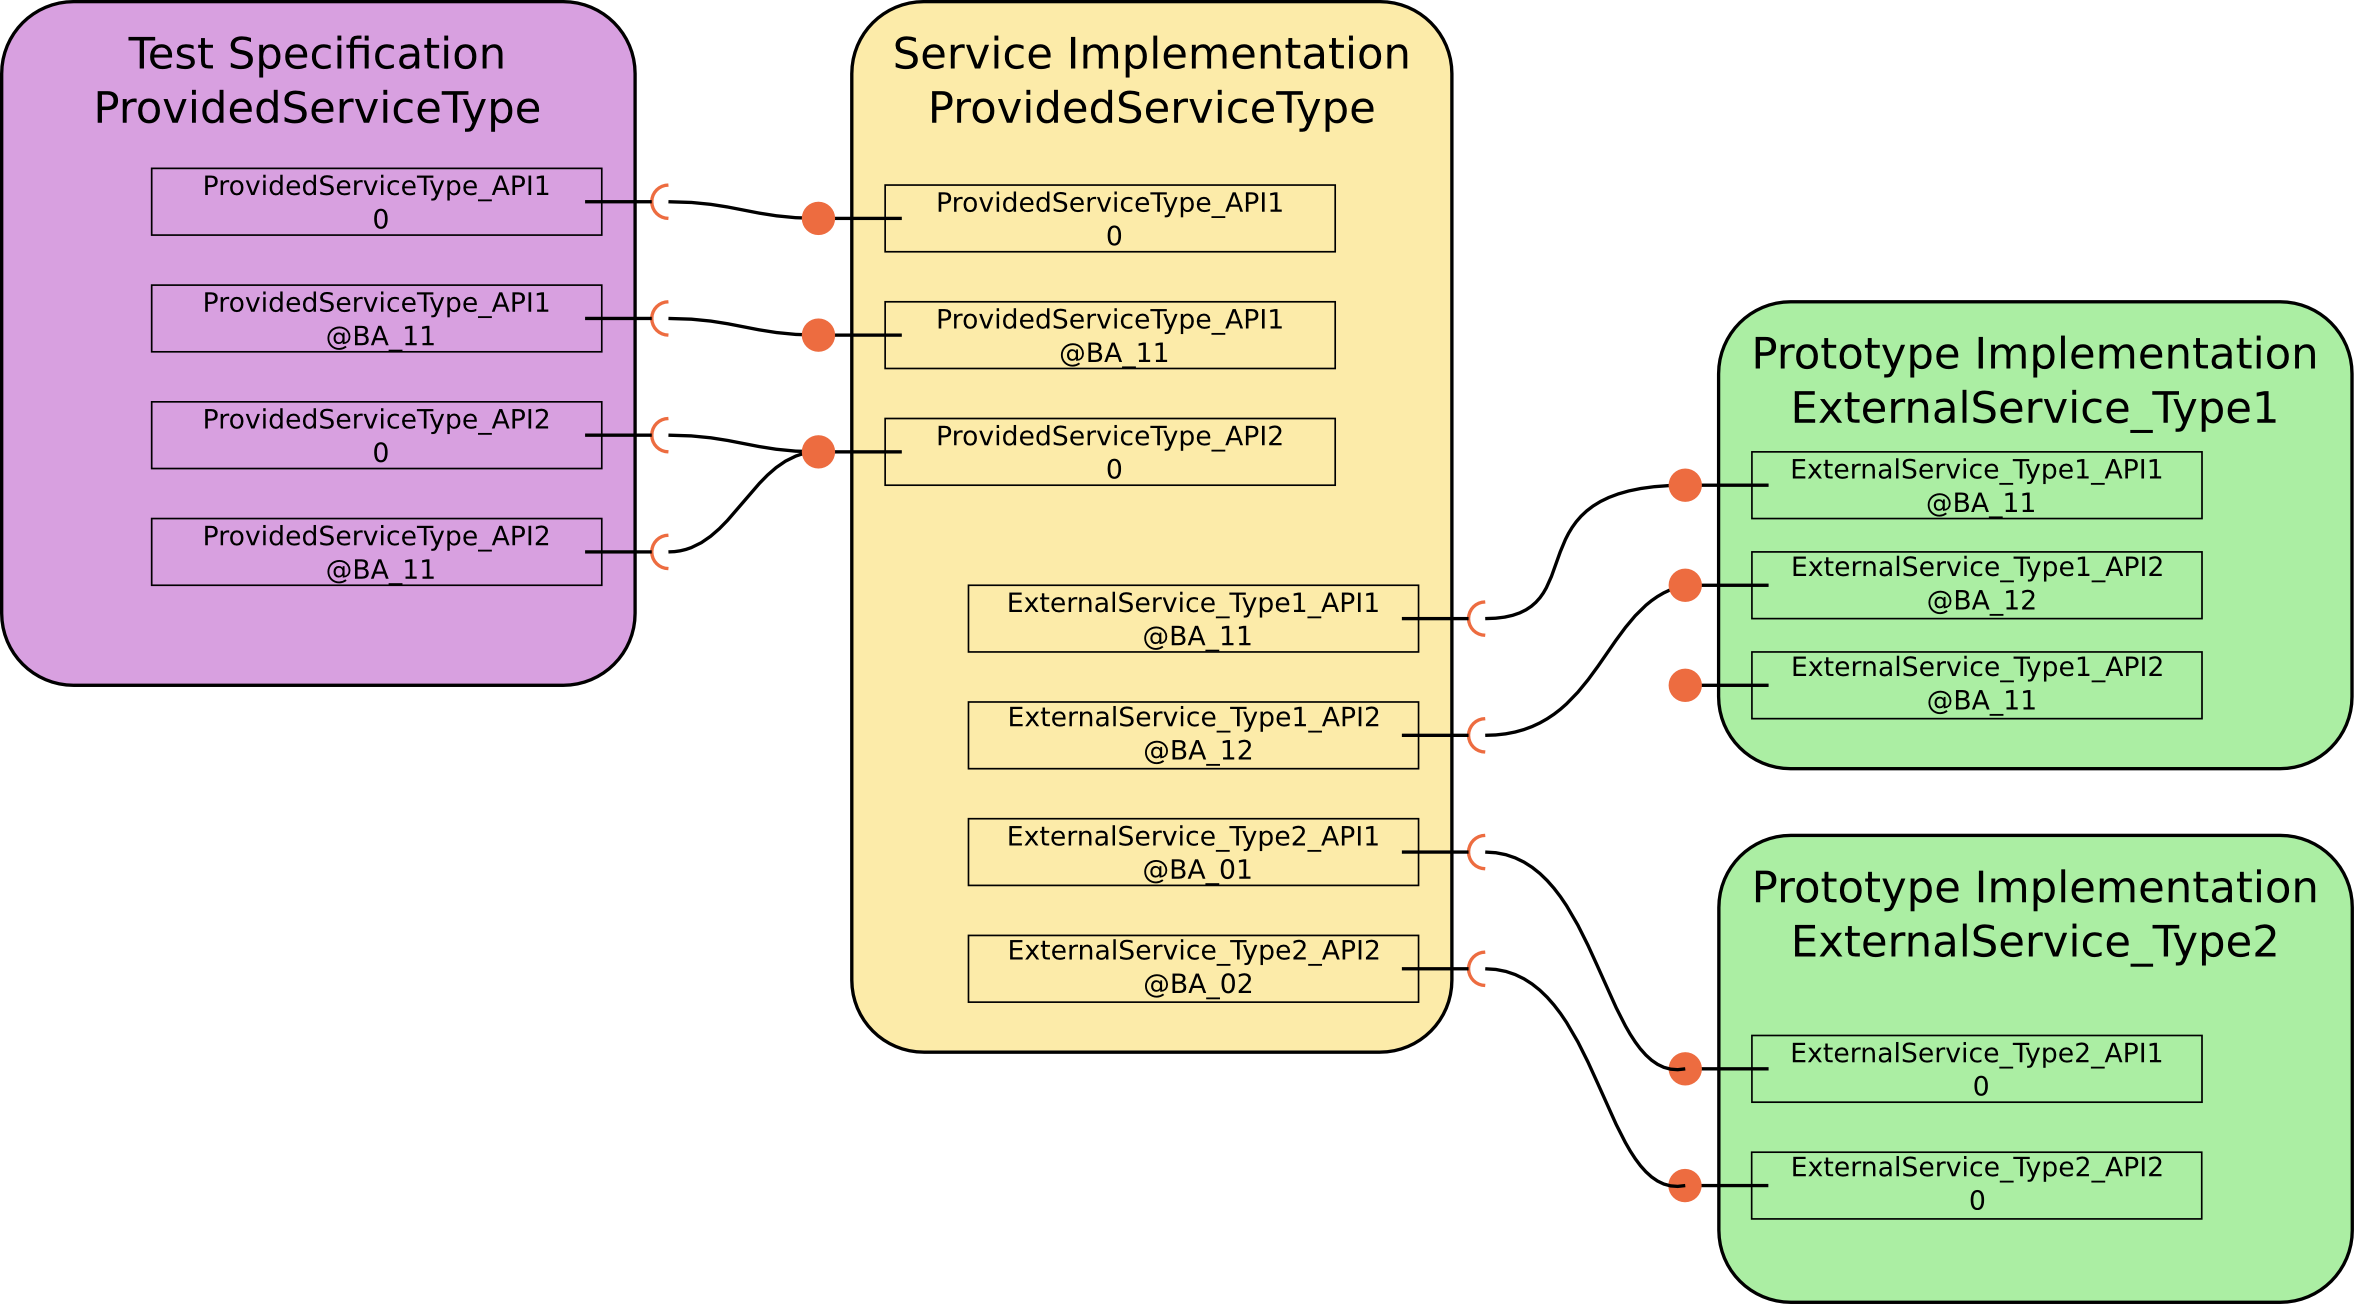
\includegraphics[width=1\textwidth]{servicePicture}
 \label{fig:serviceImplementation}
\end{figure}
Implementacje usług oraz injektowanie instancji usług
\end{frame}


\section{Architektura usługowa - Protokoł kanoniczny}
\subsection{Problemy}
\begin{frame}
Standardowe narzędzia DI nie odpowiadają architekturze usługowej. Problemy:
\pause
 \begin{enumerate}
  \item<2-> Moduł/Komponent to \emph{NIE} instancji usługi:
  \begin{enumerate}
   \item Sztywne połączenie
   \item Instancie to singletony
  \end{enumerate}
  \item<3-> Kontekst uruchomienia
  \begin{enumerate}
   \item Ograniczenie do jednej JVM
   \item ograniczenia dostępu
   \item ``własność'' usługi
  \end{enumerate}
 \end{enumerate}
\end{frame}

\subsection{Rozwiązanie - dynamiczne łączenie modułów}
% % % 
\begin{frame}{ExternalBindingSwitch}
Instancja usługi to moduł uruchomiony z ``przełącznikiem`` na potrzebne usługi:
\begin{figure}
        \begin{subfigure}[b]{0.3\textwidth}
                \centering
                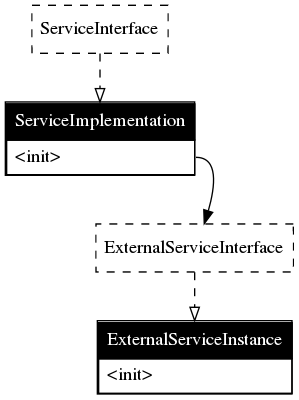
\includegraphics[width=\textwidth]{directBinding}
                \caption{Direct}
        \end{subfigure}%
        \begin{subfigure}[b]{0.3\textwidth}
                \centering
                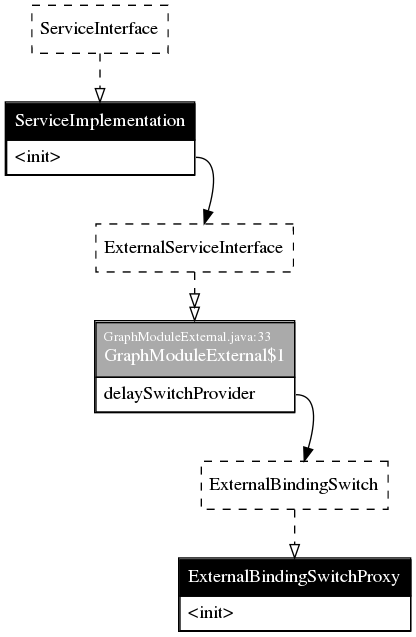
\includegraphics[width=\textwidth]{switchBinding}
                \caption{Switch}
        \end{subfigure}%
\end{figure}
\end{frame}


\subsection{Rozwiązanie - zdalne łączenie modułów}

\begin{frame}{Protokoł kanoniczny}
\begin{figure}
 \centering
 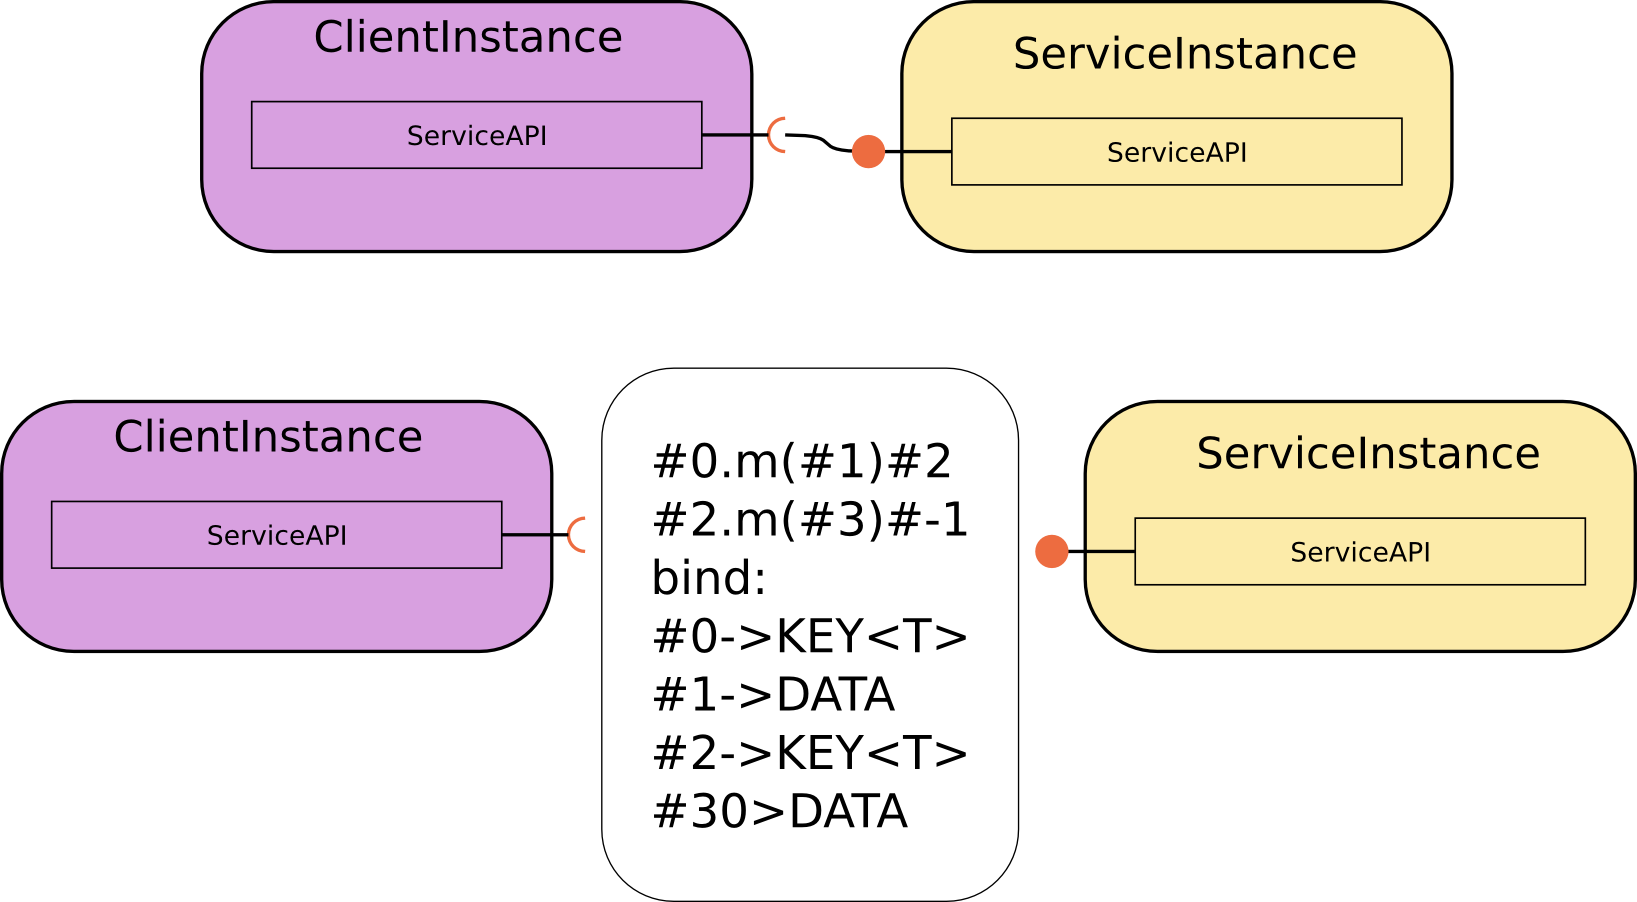
\includegraphics[width=1\textwidth]{canonicalSplit}
 \label{fig:serviceImplementation}
\end{figure}
\end{frame}

\section{Demo}
\begin{frame}{DEMO}
\begin{figure}
 \centering
 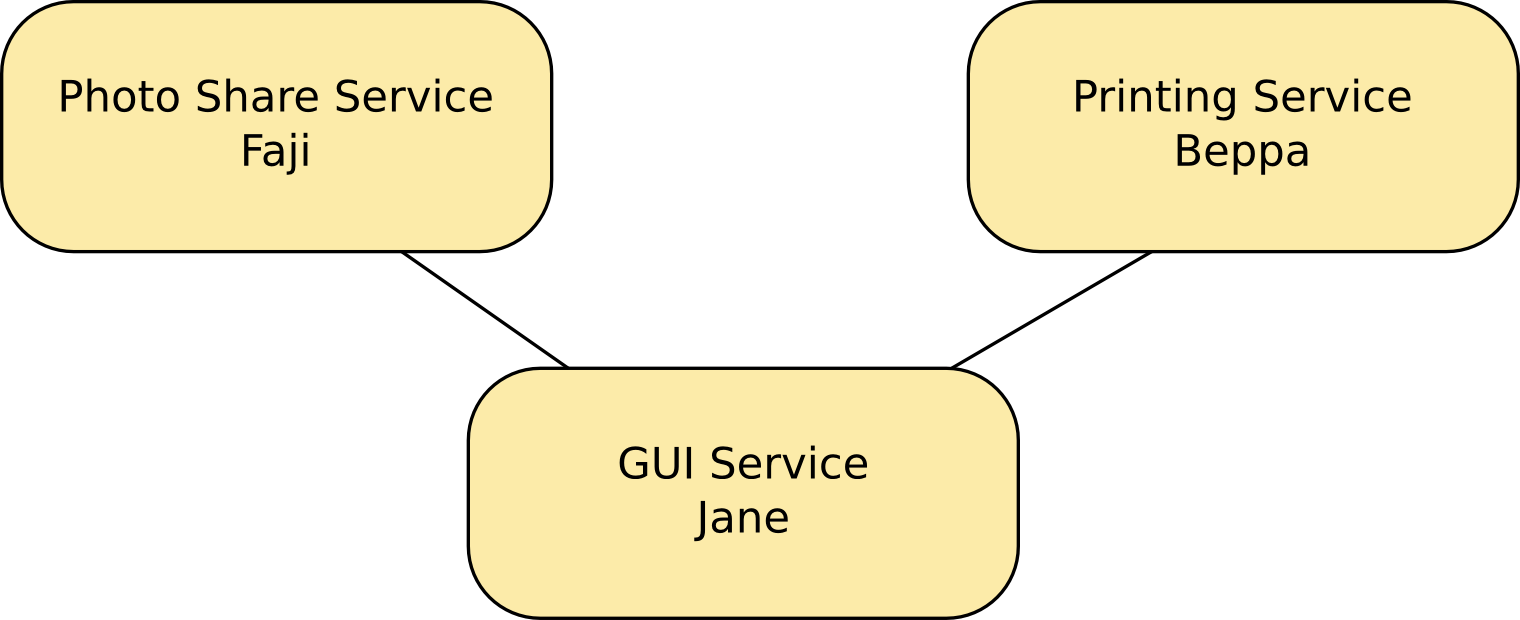
\includegraphics[width=1\textwidth]{aouthScenario}
 \label{fig:serviceImplementation}
\end{figure}
\end{frame}

% \section{Argumentacja innowacyjności SAM}
% \subsection{Nowe rozwiązanie?}
% \subsection{Why Functional Programming Matters}
% \subsection{Modularize and Glue in SAM}


\end{document}
